\documentclass{VUMIFPSkursinis}
\usepackage{algorithmicx}
\usepackage{algorithm}
\usepackage{algpseudocode}
\usepackage{amsfonts}
\usepackage{amsmath}
\usepackage{bm}
\usepackage{caption}
\usepackage{color}
\usepackage{float}
\usepackage{graphicx}
\usepackage{listings}
\usepackage{float}
\usepackage{subfig}
\usepackage{wrapfig}
\usepackage[hidelinks]{hyperref}
\usepackage{todonotes}


% Titulinio aprašas
\university{Vilniaus universitetas}
\faculty{Matematikos ir informatikos fakultetas}
\department{}
\papertype{Profesinės praktikos ataskaita}
\title{Profesinės darbo praktikos įmonėje EPAM sistemos ataskaita}
\titleineng{Report on Professional Work Practice in the Company EPAM systems}
\status{2 kurso studentas}
\author{Matas Savickis}
\supervisor{Karolis Petrauskas, Doc., Dr.}
\reviewer{Nerijus Tenys}

\date{Vilnius – \the\year}

% Nustatymai
% \setmainfont{Palemonas} % Pakeisti teksto šriftą į Palemonas (turi būti įdiegtas sistemoje)
\bibliography{bibliografija}

\begin{document}
\maketitle
\addtocounter{page}{1}
\tableofcontents

\section{Įvadas}
	\subsection{Praktikos vienos pasirinkimo motyvacija}
		Pasirinkau atlikti praktiką įmonėje EPAM sistemos, nes norėjau įgauti patirties dirbant tarptautinėje
		korporacijoje dirbant su trumpalaikiais klientų užsakymais.
	\subsection{Praktikos užduotis}
		\begin{itemize}
			\item{Vykdyti sistemos projektavimo veiklas.}
			\item{Vykdyti sistemos kūrimo veiklas.}
			\item{Vykdyti projekto apimties įvertinimą ir užduočių analizę.}
		\end{itemize}

	\subsection{Praktikos tikslas}
		Pritaikyti teorines ir praktines žinias apie programų sistemų kūrimą, įgytas Vilniaus universitete realiems projektams.

	\subsection{Spręsti praktikos uždaviniai}
		\begin{itemize}
			\item{Suprojektuoti duomenų bazės schemą.}
			\item{Išrinkti Java programavimo karkasą tinkamą debesijos kompiuterijai.}
			\item{Suprojektuoti duomenų sinchronizavimo architektūrą tarp atskirų duomenų bazių.}
			\item{Projektui parinkti kokybės užtikrinimo gerąsias praktikas ir jų vykdymo užtikrinimo būdus.}	
		\end{itemize}
	\subsection{Praktinės veiklos planas}
		Praktinė veikla truko nuo 2021-09-01 iki 2021-11-30
		\begin{enumerate}
			\item{Įvadas į projektą, naudojamus įrankius ir bendrą įmonės veiklą: 2021-09-01 iki 2021-09-10}
			\item{Praktikos užduočių atlikimas: 2021-09-11 iki 2019-11-30}
		\end{enumerate}

\section{Įmonės apibūdinimas}
	\subsection{Įmonės veiklos sritis}
		EPAM sistemos yra Baltarusijos ir Amerikos informacinių technologijų įmonės kuri specializuojasi užsakomaisiais
		projektais ir konsultavimu informacinių technologijų srityje. 		
		
	\subsection{Įmonės organizacinė struktūra}
		Įmonės padalinys Lietuvoje buvo įsteigtas prieš metus. 
		Šiuo metu įmonėje dirba apie 300 darbuotojų ir šis skaičius vis auga. 
		Didžioji dalis darbuotojų yra atvykusių iš Baltarusijos.
		Nors įmonė turi sąlyginai daug darbuotojų tačiau tik maža jų dalis būna ofise.
		Ofise dažniausiai būna apie 50 žmonių.
		Darbuotojai norėdami atvykti į ofisą turi užsirezervuoti darbo vietą vidinėje įmonės sistemoje, nes individualių
		darbo vietų nėra.
		Mano komandoje dirbo 6 žmonės.
		
	\subsection{Įmonės teikiamos paslaugos}
		\begin{enumerate}
			\item{
			Klienų programavimo projektų vykdymas - pagrindinė įmonės veiklos sritis yra klietų informacinių technologijų
		projektų vykdymas. Klientas ateina su prašymu atlikti projektą, EPAM įvertina kiek projektas kainuotų klientui
			ir pateikia pasiūlymą. Jeigu klientui tinka pasiūlymas ir nurodyti kaštai EPAM savo vidinėje sistemoje 
			suranda reikiamos kompetencijos darbuotojus atlikti projektui. Jeigu reikia surasti darbuotojai praeiną
			darbo pokalbius pas klientą.
			Praėjus darbo pokalbius EPAM darbuotojas pradeda dirbti pas klientą.
			Pats EPAM darbuotojas gali nesutikti dirbti jam siūlomame projekte jeigu tas projektas jo nedomina.
			}
			
			\item{
			Klientų konsultavimas informacinių technologijų klausimais - panašiom sąlygom kaip ir buvo minėta apie
			projektų vykgdymą, įmonė klientams teikia konsultavimo paslaugas, kuomet EPAM darbuotojas trumpą laiką
			atlieką kliento konsultavimą informacinių technologijų projektų klausimais.
			Konsultantas gali padėti įvertinti projekto apimtis, patarti kokių kompetencijų specialistų reikės,
			įvertinti reikiamą biudžetą ir panašius su projekto pradžia ar tolimesniu vystymu susijusiais klausimais.		
			}
		\end{enumerate}
	\subsection{Darbo sąlygos}
			Įmonė yra įsikūrusi Vilniuje Šeimyniškių g. 19-601.
			Pastatas yra patogioje miesto vietoje į kurią yra patogus susisiekimas viešuoju transpotu.
			Kompanija suteikia keletą nemokamo parkavimosi vietų, o kai jos pasibaigia netoliese yra nebrangios mokamos
			parkavimosi vietos.
			Ofise nėra asmeninių darbo vietų, todėl norint atvykti ir dirbti reikia užsirezervuoti darbo vietą vidinėje
			įmonės sistemoje.
			Įmonė leidžia dirbti iš namų, net ir šiuo metu kai karantino sąlygos leidžia dirbti iš ofiso.
			Per beveik metu kai dirbu šioje įmonėje ofise buvau tik keletą kartų ir jokių nusiskundimų dėl to neišgirdau.
			Darbuotojams dirbti iš namų yra suteikiama beveik visa reikalingą įranga(nešiojamas kompiuteris, monitorius, pelė ir kita).
			Pradėjęs dirbti įmonėje mėnesį praleidau vidiniame įmonės darbuotojų apmokymo procese, kuriame galėjau 
			gintis savo programavimo žinias, bei buvau apmokomas kaip sėkmingiau praeiti kliento darbo pokalbio procesą, 
			kokių klausimų dažniausiai klausiama per darbo pokalbius ir kaip į juos atsakyti teisingai.
			Po mėnesio man buvo paskirtas projektas, kuriu darbo pokalbį sėkmingai praėjau ir pradėjau dirbti kliento projekte.
		
		
\section{Praktikos veiklos aprašymas}
	\subsection{Projektas}
		Aš dirbau prie Amerikos įmonės Vertex vienkartinio prisijungimo projekto. Įmonė Vertex specializuojasi mokesčių
		skaičiavimo programinės įrangos kūrime. Vertex parduodami produktai turi daug modulių į kuriuos galima prisijungti skirtingai būdais, su skirtingais prisijungimo duomenimis. Mūsų projekto tikslas buvo sukurti vienkartinio 
		prisijungimo sistemą(angl. Single Sign-On) apjungiačia visus esamus prisijungimo būdus.
		Komandoje dirbo šeši žmonės: Viena projekto vadovė, keturi programuotojai ir vienas testuotojas.
		
	\subsection{Darbo procesas}
		Darbas šiame projekte vyko pagal Agile metodologiją.
		Kiento produkto savininkas(angl. product owner) arba sistemos architektas pateikdavo reikalavimus(angl. Epics) 
		į užduočių valdymo platformą Atlasian. Mūsų komanda iš pateiktų reikalavimų sukurdavo istorijas(angl. Stories),
		kurias mes įvertindavome kiek laiko užtruktų atliktį kiekvieną istoriją.
		Kas dvi savaite mūsų komanda suplanuodavo sprintą(angl. Sprint) ir įvertindavo kiek užduočių galės atlikti per ateinančias dvi savaites.
		Po dviejų savaičių vienas komandos narys pristatydavo kokius darbus pavyko atlikti per dviejų savaičių sprintą ir pademonstruodavo progresą kliento projektų vadovei.
		Prieš kito sprinto planavimą komanda atlikdavo savo vidinę retrospektyvą ir padiskutuodavo kas buvo gerai ir ką reiktų tobulinti, kad ateities sprintai būtų produktyvesni.
		Sprinto metu komanda darbo trumpos penkiolikos minučių susitikimus su klientų papasakoti ką kiekvienas komandos
		narys radė praeitą dieną ir ką planuoją nueikti kitą dieną.
		Šio susitikimo metu taip pat išsprendžiamos problemos dėl dabartinio sprinto užduočių.entity
		Sprinto metu programuotojai atilikinėja suplanuotas užduotis ir atlikinėja kitų komandos narių kodo peržiūras.
		Testuotojas sprinto metu atlikinėja esamo funkcionalumo testavimą ir suradęs klaidą sukurią klaidos aprašą ir užduotį Atlasian sistemoje.
		Rastas klaida kode būna pataisoma esamo sprinto metu, įtraukiama į kito sprinto planavimą arba ignoruojama ir 
		neatliekama.
		Kas atsitiks su rasta klaida nusprendžia pati komanda arba kliento architektas įvertinęs klaidos svarbumą ir kitas prioritetines užduotis.
		
	\subsection{Naudotos technologijos}
		Projekte buvo naudotas Micronaut 3 karkasas su Java 17 programavimo kalba.
		Duomenų sluoksniui kurti buvo pasirinkta reliacinė MySQL duomenų bazė ir objektų ryšių suvedimo biblioteka Hibernate.
		Programa buvo kuriama pagal REST API standartą. Aprašyti REST specifikacijai buvo naudojama OpenAPI specifikacijų kalba.
		Autorizacijai ir autentifikacijai mūsų komanda naudojo Auth0 platformą siekiant užtikrinti saugumą, palengvinti projekto įgyvendinimą ir sumažinti projekto 
		biudžetą.
		Užtikrinti kodo kokybę mes naudojome įvarius statinio kodo analizės įrankius, tokius kaip: PMD, SpotBug, Checkstyle, Depedency Checker, Pom-lint.
		Visi šie statiniai kodo analizatoriai padėjo užtikrinti, kodo kokybę, tvarką ir saugumą.
		
	\subsection{Užduotis: Suprojektuoti duomenų bazės schemą.}
		Pradedant projekta klientas pateike verslo reikalavimus, kaip skirtingi mokesčiu modeliai saveikauja tarpusavyje ir kokias reikšmes jie turi.
		Reikejo sukurti duomenu bazes schema kuri pasižymetų šiomis savybėmis:
		\begin{itemize}
			\item{Esybė turėtų švelnaus užrakinimo (angl. Soft lock) savybė.}
			\item{Kiekvienas esybė turėtų unikalų identifikatorių.}
			\item{Būtų įmanoma pasakyti kada esybė buvo sukurta.}
			\item{Būtų įmanoma pasakyti kada esybė buvo atnaujinta.}
		\end{itemize}

		Pagal pateiktus reikalavimus buvo sudaryta duomenų bazės schema.

		ČIA BUS SCHEMA KAI NETYNGESIU JA IKELTI

		Kiekviena schemos esybė paveldi iš tėvinės BaseEntity esybės kuri turi šiuos laukus
		\begin{itemize}
			\item{Id(UUID) - unikalus esybės identifikatorius UUID formatu užtikrinančiu, kad duplikatinio UUID tikimybė yra arti nulio.}
			\item{Version(Integer) - inkrementaliai didėjantis skaičius kartu su Hibernate karkasu užtikrinantis švelnaus užrakto(angl. Soft lock) fukcionalumą.}
			\item{CreatedAt(Date) - datos formatas parodantis kada esybė buvo sukurta}
			\item{UpdatedAt(Date) - datos formatas parodantis kada esybė buvo pakeista paskutinį kartą.}
		\end{itemize}


		\begin{figure}[H]
			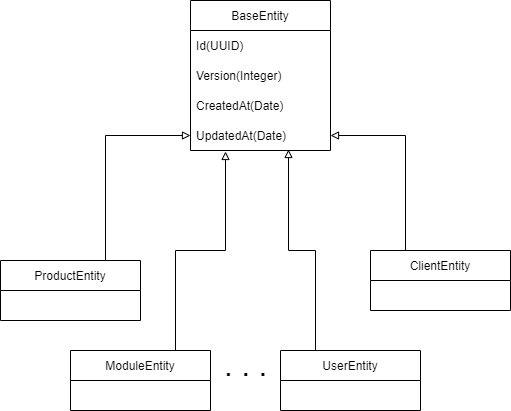
\includegraphics[scale=0.7]{img/eight}
			\caption{Duomenų bazės esybių paveldėjimo diagrama} % Antraštė įterpiama po paveikslėlio
			\label{img:kurimoProcesas}
		\end{figure}

		Projekte buvo naudojama MySQL duomenų bazė pagal kliento prašymą.
		Atlikti duomenų bazės pakeitimų migracijai buvo naudojama Liquibase migracijų įrankis.

	\subsection{Užduotis: Išrinkti Java programavimo karkasą tinkamą debesijos kompiuterijai.}
		Projektą pradėjome nuo pradžių ir gavome iš kliento prašymą išrinkti Java kalbos karkasą labiau pritaikyą debesijos skaičiavimams.
		Paprastas sprendimas būtų buvęs pasirinkti šiuo metu populiariausią Spring karkasą ir jį naudoti, tačiau norėjome įsitikinti, ar jis yra geriausias pasirinkimas.
		Atlikus pirmine analize supratome, kad Spring karkasas turi dvi pagrindines problemas
		\begin{itemize}
			\item{Ilgas šalto paleidimo laikas(angl. Cold start).}
			\item{Didelis sugeneruotu failu dydis.}
		\end{itemize}
		Abu šie paminėti aspektai apkrauna debesijos aplinką, ko pasekoje debesijos paslaugos kainuoja daugiau, ypač jeigu sistemoje yra šimtai tinklo mazgų.
		Atlikus paiešką internete buvo prieita prie alternatyvų Spring karkasui:
		\begin{itemize}
			\item{Micronaut}
			\item{Quarkus}
		\end{itemize}
		Abu šie karkasai pasižymi priešlaikiniu kompiliavimu(angl. Ahead of Time Compilation).
		Šis kompiliavimo būdas leidžia sukompiliuoti aukšto lygio programinį kodą į vietinį baito kodą(angl. Native byte code).
		To deka vietiniai faila būna mažesnio dydžio negu kompiliuojant tradiciniu pačiu laiku kompiliavimu(angl. Just In Time compilation).
		Kadangi atliekamas priešlaikinis kompiliavimas programai nereikia atlikti daug resusų kainuojančių refleksijos operacijų sulėtinančių programos paleidimą.
		Vietiniai failai taip pat leidžia naudoti vietinių failų virtualias mašinas tokias kaip GraalVM kurių dėka paleidimo greitis yra sumažinamas.
			\begin{figure}[H]
			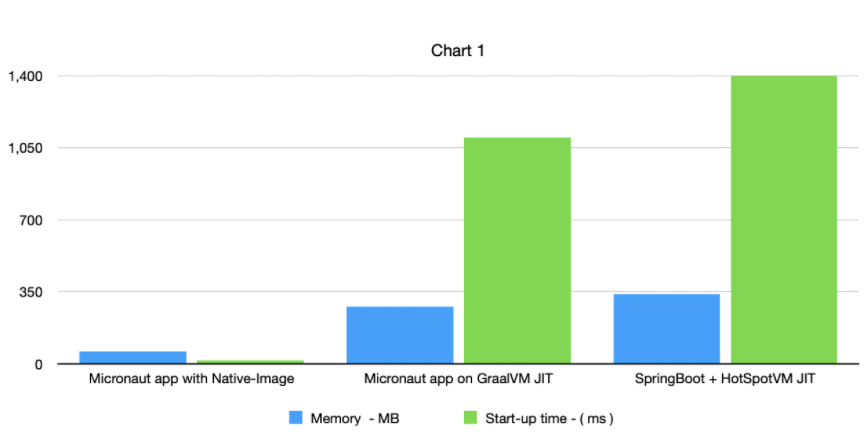
\includegraphics[scale=0.7]{img/three}
			\caption{Spring ir Micronaut palyginimas naudojant GraalVM} % Antraštė įterpiama po paveikslėlio
			\label{img:kurimoProcesas}
			\end{figure}
			\begin{figure}[H]
			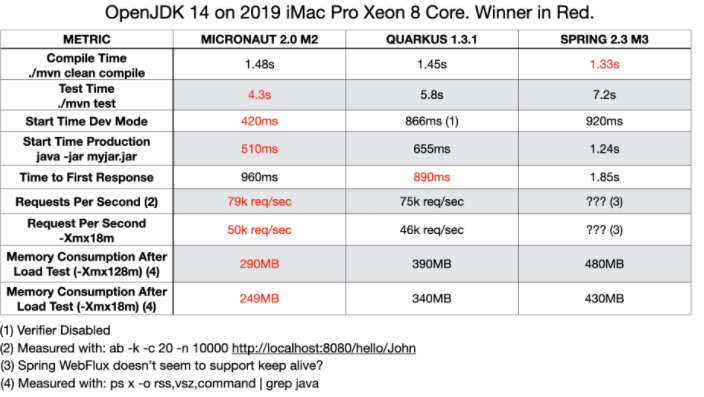
\includegraphics[scale=0.85]{img/one}
			\caption{Spring, Micronaut ir Quarkus palyginimas} % Antraštė įterpiama po paveikslėlio
			\label{img:kurimoProcesas}
			\end{figure}
			\begin{figure}[H]
			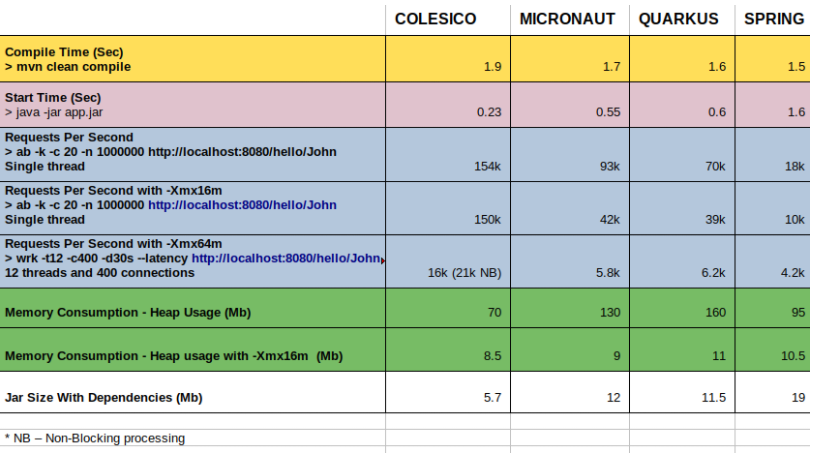
\includegraphics[scale=0.7]{img/two}
			\caption{Spring, Micronaut, Quarkus ir Colesico palyginimas} % Antraštė įterpiama po paveikslėlio
			\label{img:kurimoProcesas}
			\end{figure}
		Palyginus internete rastus testus matuojancius Spring, Micronaut ir Quakus kompiliavimo laiką, atminties sunaudojimą, pasileidimo greiti ir užklausu apdorojimo greitį
		matome, kad Micronaut ir Quarkus karkasai skiriasi nežymiai, vienuose testuose laimi Micronaut, kituose Quarkus, tačiau matomas  skirtumas tarp šiu dvieju karkasu ir Spring karkaso.
		Spring karkasas laimi tik kompiliavimo greičio kategorijoje, kas produkciniai aplinkai nėra svarbu.
		Nusprendeme pasirinkti Micronaut karkasa, nes jis savo sintakse yra panašus Spring karkasui ir komanda jau turejo patirties dirbant su Spring.
		Beto, jeigu ateityje Spring karkaso kūrėjai įgyvendins prieškaikinį kompiliavimą ir ir vietinių failų kūrimą bus nesunku migruoti projekta atgal į Spring.


	\subsection{Užduotis: Suprojektuoti duomenų sinchronizavimo architektūrą tarp atskirų duomenų bazių.}
		Kurdami integraciją su Auth0 servisu turejome užtikrinti, kad duomenys tiek Auth0 duomenų bazėje tiek kliento duomenų bazėje sutaptu.
		Tiek bandant įrasyti duomenis į Auth0 duomenų bazę tiek į kliento vidinę duomenų bazę(toliau Vertex duomenų bazė) gali ištikti sutrikimai, kurių metu duomenys neišsisaugotu ir atsirastų nesutapimas tarp šiu baziu.
		Gali įvykti 
		Kadangi duomenys bandomi irasyti i dvi skirtingas duomenu bazes neimanoma visko atlikti per viena tranzakcija.
		Reikia sugalvoti mechanizma uztikrinanti, kad ivykus sutrikimui, duomenys butu atstatomi sutrikimo metu, o atstatyti nepavykus pranešti palaikymo komandai, kad duomenys būtų pataisyti rankiniu būdu. 
		Kuriant tokį mechanizmą svarbu įgyvendinti šiuos scenarijus:
			\begin{figure}[H]
			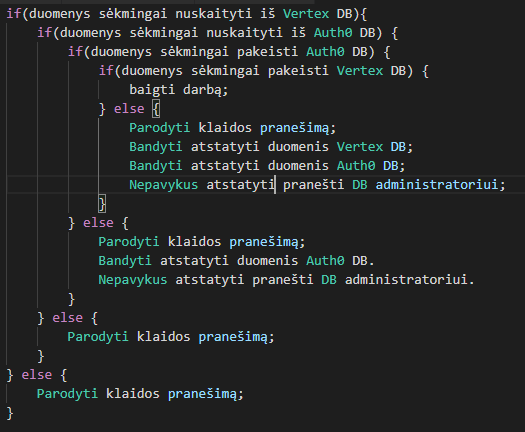
\includegraphics[scale=0.7]{img/five}
			\caption{Sinchronizavimo mechanizmo pseudokodas} % Antraštė įterpiama po paveikslėlio
			\label{img:kurimoProcesas}
			\end{figure}
		Kaip matome kuriant funkcionalumą paprastai kodas tampa labai komplikuotas, sunkiai skaitomas ir palaikomas.
		Taip pat atliekant operacijas su skirtingom klasėm atsiranda kodo duplikacijos.
		Šį pseudo kodą galima perdaryti į skaitomesni ir bendresni kodą:
			\begin{figure}[H]
			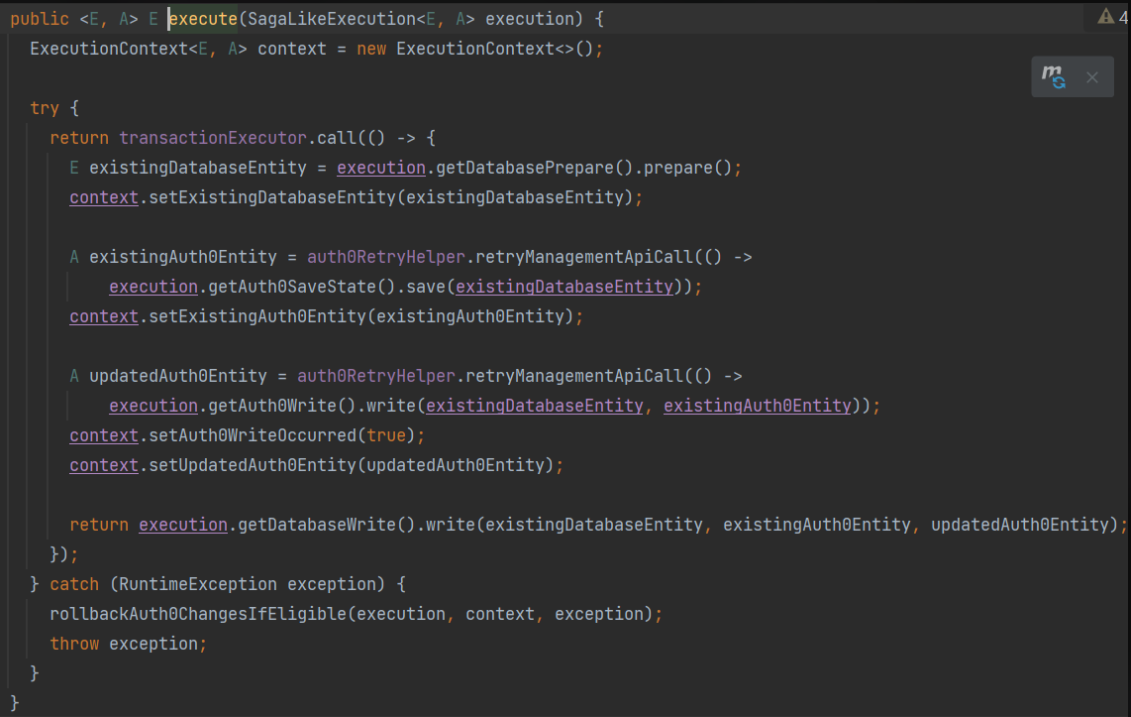
\includegraphics[scale=0.5]{img/six}
			\caption{Sinchronizavimo mechanizmo įgyvendinimas} % Antraštė įterpiama po paveikslėlio
			\label{img:kurimoProcesas}
			\end{figure}

		Naudojant šį kodą atlikti duomenų sinchronizacimui atrodytu taip:

			\begin{figure}[H]
			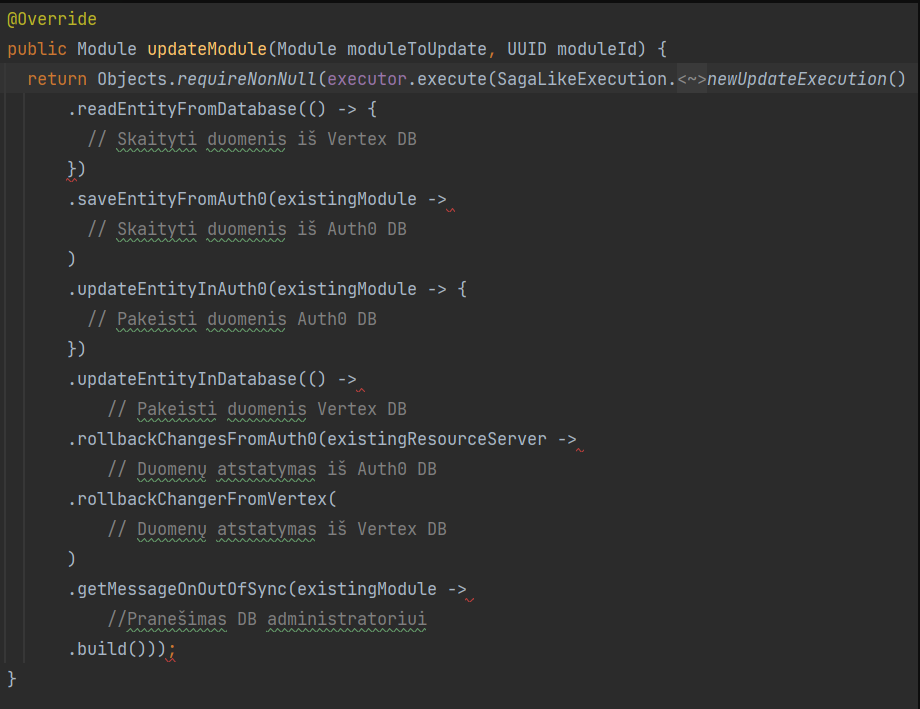
\includegraphics[scale=0.7]{img/seven}
			\caption{Sinchronizavimo mechanizmo panaudojimas} % Antraštė įterpiama po paveikslėlio
			\label{img:kurimoProcesas}
			\end{figure}

		Šiuo metu pademonstruotas kodas yra sėkmingai naudojamas projekte.
		Sinchronizavimo mechanizmo pasekoje pagerėjo kodo skaitomumas, klaidų valdymas ir duomenų bazių atstatymas ištikus klaidai.
		
		


	\subsection{Užduotis: Projektui parinkti kokybės užtikrinimo gerąsias praktikas ir jų vykdymo užtikrinimo būdus.}
		Komanda nutarė, kad norime išlaikyti aukštą kodo kokybę, sumažinti kodo klaidų ir saugumo spragų.
		Norint įgyventinti šia užduotį reikia surasti reikiamus įrankius padėsiančius užtikrinti užsibrėžtus tikslus bei integruoti juos į programos kūrimo
		procesą taip, kad būtų kuo sunkiau apeiti šiuos įrankius, nes gera programuotojų valia nevisuomet galima pasitikėti.
		Užduotį pradėjau vykdyti atlikdamas įvairių statinės analizės įrankių paiešką ir įvertinimą.
		Internete pavyko rasti nemažai mokamų ir nemokamų priemonių vykdančių kodo analizę.
		
		\subsubsection{JavaDocs validacija}
			Vienas iš būdų užtikrinti sklandų kodo palaikymą ateityje, kaip prie jo dirbs kiti programuotojai yra kodo dokumentacija.
			Dažnai projektuose nutinka taip, kad dokumentacija būna daroma atmestinai arba jos išvis nebūna ir kitai komandai perėmus projektą prireikia daug 
			laiko ir pastangų toliau vystyti projektą.
			Dėl šių priežasčių komanda nutarė, kad dokumentacijos rašymas turi būti integruotas į programų kūrimo procesą.
			Vienas iš būdų Java kode rašyti dokumentacija yra naudoti Javadocs dokumentų generatorių kurio pagalba atitinkami Java kodo komentarai būtų 
			sugeneruoti į dokumentaciją. 
			Užtikrinti, kad JavaDocs komentarai būtų rašoma kiekvienam viešam klasės metodui ir kontraktui naudosime  maven-javadocs-plugin biblioteką, kuri užtikrina, kad visi komentarai būtų rašomi tinkamu formatu, visų reikiamų metodų ir kontraktų parametrai būtų nurodyti ir aprašyta ką daro kiekvienas iš metodų.
			Jeigu vienas iš nurodytų kiterijų nėra įgyventintas maven-javadocs-plugin parodo klaidą ir pasako ko trūksta kad dokumentacija būtų teisinga.
			\begin{figure}[H]
			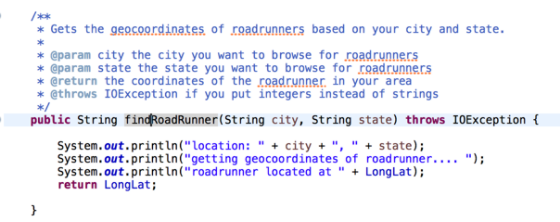
\includegraphics[scale=0.7]{img/four}
			\caption{JavaDocs pavyzdys} % Antraštė įterpiama po paveikslėlio
			\label{img:kurimoProcesas}
			\end{figure}
		\subsubsection{PMD}
			Gero kodo požymis yra kai jame laikomasi tvarkos: nėra nepanaudotų kintamūjų ar nenaudojamų bibliotekų, kintamūjų pavadinimai turi prasmę ir laikomasi jų pavadinimo standartų, kode nėra magiškų skaičių(angl. Magic number). Dažnai tokius dalykus galima pastebėti kodo peržiūros stadijoje, tačiau visi žmonės klysta ir kartais praleidžia šiuos dalykus pro pirštus, beto jeigu būtų įrankis galintis patikrinti šiuos dalykus kodo peržiūros užimtų mažiau laiko.
			Vienas iš atviro kodo įrankių plačiai naudojamos tokio tipo statiniai kodo analizei yra PMD. Jo pagalba galima patikrinti didelę aibę kodo stiliaus klaidų, gerūjų praktikų trūkumų bei daug kitų panašių dalykų.
			PMD turi savų trūkumų, kartais yra rodomos klaidos kurių negalima ištaisyti, pavyzdžiui rodomos klaidos naudojant Lombok generuojamą kodą.
			Išspręsti tokius tūkumus padeda lanksti PMD konfigūracija, kurios pagalba galima išjungti norimas kodo analizės taisykles visam projektui arba tik vienam failui.
		\subsubsection{SpotBugs}
			SpotBugs yra statinės kodo analizės įrankis padedantis surasti kodo klaidas, tokias kaip neinicializuoti laukai, laukai turintys null reikšmę kai kode anotacijos null reikšmės neleidžia, sąlygos sakiniai visuomet gražinantys tą pačia reikšmę bei kitas klaidas kurios sintaksiškai yra teisingos, bet gali sukelti programos sutrikimus ateityje.
		\subsubsection{Kodo priklausomybių tikrinimas}
			Siekiant užtikrinti, kad projekto kodas būtų saugus svarbu užtikrinti, kad kode naudojamos priklausomybės būtų saugios.
			Šiam tikslui naudojome dependency-check-maven ir maven-enforcer-plugin bibleotekas, jos užtikrino, kad naudojamos kodo priklausomybių versijos neturi žinomų saugumo spragų ir priklausomybių versijos nesiduplikuoja arba nėra nurodytos dvi skirtingos versijos tai pačiai priklausomybei.
		\subsubsection{Checkmarx ir SonarQube}
			Kliento prašymu turėjome naudoti Checkmarx saugumo statinį analizatorių ir SonarQube statinių kodo analizatorių.
			Kaikurie dalykai analizuojami šių įrankių jau buvo daromi aukščiau minėtuose įrankiuose, bet buvo nutarta palikti naudojamus įrankius, nes jų vykdymo laikas yra trumpesnis ir perteklinė analizė nėra blogai.
		\subsubsection{Vieneto ir integraciniai testai}
			Dar vienas svarbus kodo kokybės aspektas yra testai.
			Nutarėme, kad projekto išeities kodas turi būti 80 procentų padengtas testais.
			Tą užtikrinti naudojome Jacoco biblioteką parodančia koks yra projekto kodo padengimo testais procentais.
			Jacoco biblioteka skaičiuoja kiek Java baitų kodo eilučių pasiekia testai.
		\subsubsection{Kodo formatavimas}
			Paskutinis aspektas kurį norėjome užtikrinti buvo kodo stiliaus pastovumas.
			Jeigu kodas visame projekte atrodo panašiai tampa lengiau skaityti ir suprasti kodą.
			Šiam tikslui pasirinkome plačiai naudojama Google Java style konvenciją, kurią tikrinom pagal Google suteiktą stiliaus tikrinimo įrankį checkStyle. 
		\subsubsection{Integracija su Github Actions}
			Suprantome, kad reikia priversti programuotojus naudotis statinio kodo analizės įrankiais nes kitu atveju niekas jų nenaudos.
			Buvo nutarta šiuos įrankius sukonfigūruoti Github Action aplinkoje, kuri užtikrina, kad joks kodas negalėtų patekti į kodo bazę prieš tai nepraėjęs visų minėtų įrankių.
			Visi šie įrankiai kartu su Github Actions integracija yra toliau sėkmingai naudojami komandoje.
		\subsubsection{Rezultatai}
			Pradėjus naudoti visus aukšiau minėtus įrankius kilo kėblumų, įrankiai rodė kodo klaidas kur jų nebuvo, kai kurių kodo klaidų
			nebuvo įmanoma pataisyti, nes jos kilo iš generuojamo kodo(pavyzdžiui  naudojant Lombok biblioteką).
			Tačiau praėjus kiek laiko konfigūracija buvo pritaikyta komandos poreikiams ir kodas atrodo labai švariai ir tvarkingai.
			Sėkimingai surandamos kodo klaidos ir saugumo spragos.

		
\section{Rezultatai, išvados ir pasiūlymai}
	\subsection{Rezultatai}
		\begin{itemize}
			\item{Suprojektuota ir įgyvendinta duomenų bazės schema.}
			\item{Įvertinti Java kalbos karkasai ir išrinktas karkasas leidžiantis greitesnį šaltą paleidimą(angl. Cold start) ir mažesnius failo dydžius.}
			\item{Sėkmingai suprojektuotas ir įgyvendintas duomenų sinchronizavimas tarp dviejų duomenų bazių.}
			\item{Išrinktos ir integruotos kodo analizės priemonės pagerinančios kodo kokybę ir projekto saugumą.}
			\item{Pagilinti darbo komandoje įgudžiai.}
			\item{Susipažinta su projektinių įmonių darbo praktika.}
		\end{itemize}
		
	\subsection{Išvados}
		Praktika įvyko sėkmingai. Jos metu išmokau naujų technologijų bei pagilinau žinias tose technologijose kurias jau mokėjau. 
		Praktikos užduotys buvo įgyvendintos sėkmingai. Sėkmingai pritaikiau teorines ir praktinias žinias įgytas universitete.
		Darbe aprašytos užduotys buvo tik dalis per praktika nuveikto darbo ir žinių kurių pasisėmiau.
		Įgytas praktikos žinias ir toliau taikysiu savo darbe ir kituose ateities projektuose.
		
	\subsection{Privalumai ir trūkumai}
		Privalumai: praplėčiau savo žinias apie REST tipo projektus, modernius programavimo karkasus, statinius kodo analizatorius ir gerasias programavimo
		praktikas. Turėjau galimybę programuoti naujausia Java kalbos versija, kas yra retas malonumas.  

		Trūkumai: Projekto metu vykdavo labai daug susitikimų su klientu, kurie atitraukdavo dėmesį nuo darbo. Informacija iš visų šių susitikimų galėdavo būt perduodama išsiuntus elektroninį laišką vietoj pačio susitikimo.

	\subsection{Pasiūlymai}
		Siūlyčiau sumažinti susitikimų trukmę ir dažnumą. Būna tokių dienų kai visas dienos darbas būna dalyvauti susitikimuose, kurie net nėra susije su mūsų 
		projekto darbu. Net jeigu susitikimai būna trumpi jie atitraukia dėmesį nuo užduočių darymo ir reikia laiko vėl susikaupti po susitikimo, kas mažina dienos produktyvumą.
		
\printbibliography[heading=bibintoc]

\end{document}


